\documentclass[12pt]{article}
\usepackage[utf8]{inputenc}
\usepackage[spanish]{babel}
\usepackage{amsmath}
\usepackage{amssymb}
\usepackage{graphicx}
\usepackage{hyperref}
\usepackage{float} % en el preámbulo
\usepackage{pdfpages}
\usepackage[numbers]{natbib}
\usepackage{subcaption}
\usepackage{tabularx}
\usepackage{booktabs}
\usepackage{array}
\usepackage{subcaption} % Permite crear subfiguras
\usepackage{comment} 
\usepackage{graphicx}
\usepackage{svg}
\addto\captionsspanish{\renewcommand{\tablename}{Tabla}}





\title{Estimación de distancias a transeúntes en entornos dinámicos mediante visión computacional monocular}
\author{Castelan Rosete Marco A. \and Tapia Acosta Uriel}
\date{\today}

\begin{document}

\begin{titlepage}
  \thispagestyle{empty} % sin número de página
  \includepdf[pages=1,offset=0 0,fitpaper=true]{portadaTT.pdf}
\end{titlepage}

\section*{Agradecimientos}


\newpage

\section*{Resumen}
``En el presente proyecto se aborda el desarrollo de un sistema de estimación de distancias a transeúntes en entornos dinámicos mediante visión computacional monocular. A partir de imágenes capturadas desde la perspectiva de un peatón, se calcularon distancias reales aproximadas aplicando un modelo geométrico basado en las propiedades ópticas de la cámara y las dimensiones de los sujetos observados. Con estos datos se conformó un conjunto de entrenamiento que permitió ajustar una red neuronal recurrente (RNN) para la predicción de distancias en secuencias de video''. 

\vspace{0.5cm}


\textbf{Palabras clave:} Estimación de distancias, objetos dinámicos, visión computacional monocular, entornos urbanos. 

\newpage

% Índice
\tableofcontents
\newpage

%%%%%%%%%%%%%%%%%%%%%%%%%%%%%%%%%%%%%%%%%%%%%%%%%%%%%%%

\section{Introducción}
\label{cap-intro}

La estimación de distancias es fundamental para el funcionamiento seguro y eficiente de sistemas móviles y autónomos, como vehículos autónomos, robots móviles y asistentes personales, y se realiza tradicionalmente mediante sistemas de imágenes estéreo, multicámara o mediciones LiDAR. Sin embargo, estos enfoques presentan limitaciones en términos de costo, casos de uso, sincronización, complejidad de equipamiento y consumo energético \cite{agand2024dmode}. En contraste, la visión monocular, potenciada por avances en aprendizaje profundo, ha emergido como una alternativa viable y más accesible, permitiendo la estimación de profundidad a partir de una única imagen RGB\cite{zhao2020monocular}.\\
En este contexto, el proyecto desarrolla y valida un sistema de estimación de distancias a partir de video monocular filmado desde la perspectiva de un peatón, integrando un enfoque geométrico que aprovecha la altura real de los sujetos y los parámetros intrínsecos de la cámara, a partir de los cuales se construyó un conjunto de datos propio; el análisis estadístico de esas mediciones mostró que características visuales como la altura en píxeles y la coordenada vertical del centro del cuadro envolvente de cada persona correlacionan de manera consistente con la distancia real, lo cual orientó la selección de entradas del modelo. Sobre esa base se diseñó y entrenó una arquitectura recurrente para realizar regresión de distancia en secuencias temporales, y se integró un detector YOLOv8, sin reentrenamiento, para localizar peatones en cada cuadro y alimentar el sistema. Los resultados experimentales, muestran la capacidad del enfoque para generalizar a personas de alturas variables en escenarios dinámicos y establecen las métricas de error y limitaciones que guían futuras mejoras.   

\subsection{Antecedentes}

La estimación de distancias hacia objetos presentes en una escena posee la particularidad de que el objeto de interés puede seleccionarse según la finalidad de la aplicación. Por ejemplo, en \cite{GuzmanSee2023} se aborda un escenario de conducción en el que las placas vehiculares son el objeto principal, dado que mantienen dimensiones físicas estandarizadas a nivel nacional. Esta característica permite calcular la distancia mediante el modelo óptico del lente y, con apoyo de un mapa de profundidad generado por MiDaS \cite{ranftl2020towards}, extrapolar distancias hacia otros objetos de la escena.

En situaciones donde los objetos presentan variaciones naturales de tamaño, es posible recurrir a medidas promedio o estandarizadas. Tal es el caso de \cite{haseeb2018disnet}, donde para cada clase de objeto se establecieron alturas y anchos promedio que, junto con cuatro características extraídas del cuadro envolvente generado por YOLO, sirvieron como entrada para una red neuronal densa con capas de 100 neuronas cada una.

Si bien los perceptrones multicapa constituyen arquitecturas simples capaces de capturar patrones relevantes y mostrar resultados satisfactorios, presentan limitaciones en entornos dinámicos donde intervienen personas en movimiento. En estos escenarios, ignoran un factor esencial que la visión humana emplea para inferir profundidad: el movimiento. Para abordar esta limitación, \cite{Wang_2019_CVPR} propone un modelo que procesa secuencias de imágenes mediante una etapa inicial convolucional seguida de capas recurrentes, integrando así información temporal relevante para la estimación de distancias.

\subsection{Planteamiento del problema}

Considerando los antecedentes mencionados previamente, se vuelve necesario precisar con claridad cuál es el desafío específico que este proyecto busca atender. En la siguientes subsecciones se presenta la definición del problema, donde se delimitan los alcances técnicos, las restricciones operativas y las condiciones bajo las cuales se pretende desarrollar una solución y por qué se considera viable.

\subsubsection{Definición del problema}

Los estudios comparativos recientes sobre modelos de estimación monocular de distancias \cite{spencer2024third} muestran una clara tendencia hacia arquitecturas generativas de gran escala, destacando a DepthAnything como el modelo basado en transformers más influyente del 2024. Este tipo de soluciones ofrece resultados altamente competitivos y, en algunos casos, admite el procesamiento de secuencias de imágenes. No obstante, su implementación requiere recursos computacionales elevados, lo cual dificulta su adopción en sistemas de bajo costo, aplicaciones móviles o contextos que demandan tiempos de respuesta reducidos.

En contraste, cuando el interés se concentra en uno o pocos objetos específicos, y estos poseen dimensiones constantes, es posible recurrir a un cálculo directo de distancia mediante las características ópticas de la cámara. Sin embargo, este enfoque obliga a utilizar siempre el mismo dispositivo de captura, limitando la escalabilidad y restringiendo el uso a un conjunto reducido de usuarios. Por otro lado, cuando los objetos presentan variabilidad de tamaño, se podría optar por emplear medidas promedio para guiar a un modelo de predicción. No obstante, cuando la variabilidad es grande, como en el caso de las personas, esta estrategia introduce incertidumbre y puede comprometer la capacidad del modelo para generalizar.

Adicionalmente, gran parte de los avances en estimación de profundidad y detección de objetos se ha desarrollado en contextos vehiculares utilizando conjuntos de datos como KITTI, Cityscapes y nuScenes, diseñados desde la perspectiva de un automóvil en movimiento y orientados a la conducción autónoma \cite{niu2021monocular}. Esto limita la aplicabilidad de los modelos a entornos peatonales o interiores, donde las dinámicas de movimiento, las distancias relevantes y la interacción con el entorno difieren. Incluso en datasets más diversos, como DIODE, suelen privilegiarse configuraciones estáticas \cite{li2024synthetic}, dejando de lado escenarios con movimiento humano natural.

Finalmente, construir un conjunto de datos propio con valores de distancia reales precisos implica recurrir a sensores especializados, como LiDAR o sistemas láser de alta precisión, cuyo costo dificulta su uso en proyectos de bajo presupuesto. Esta barrera tecnológica subraya la necesidad de explorar alternativas que permitan generar estimaciones métricas utilizando únicamente cámaras monoculares y modelos de geometría óptica capaces de lograr resultados reales y con recursos limitados.

\subsubsection{Justificación}

La necesidad de estimar distancias de manera confiable en entornos peatonales es cada vez más relevante en aplicaciones como asistencia para movilidad, sistemas de vigilancia inteligente, robots de servicio y plataformas portátiles de bajo costo. Sin embargo, la mayoría de los avances recientes en estimación de profundidad se han centrado en contextos vehiculares y modelos de gran escala que requieren capacidades computacionales sustanciales, lo que limita su uso y accesibilidad para escenarios específicos con recursos limitados.

Ante este panorama, resulta pertinente explorar alternativas que aprovechen únicamente visión monocular, ya que una cámara RGB convencional representa un sensor económico, ampliamente disponible y de bajo consumo y mantenimiento. Asimismo, el uso de modelos geométricos para generar referencias de distancia evita depender de sensores costosos como LiDAR, volviendo viable la realización de un conjunto de datos propio y adaptado al dominio peatonal.

La integración de información temporal mediante redes recurrentes ofrece además la posibilidad de capturar señales dinámicas, como cambios en tamaño aparente o desplazamiento vertical del objeto detectado, que la visión humana utiliza de manera natural para inferir profundidad. Este enfoque permite desarrollar un sistema más cercano al comportamiento perceptual humano y mejor adaptado a situaciones reales donde los sujetos están en movimiento.

\subsection{Hipótesis}

Si se integra un modelo basado en parámetros intrínsecos de la cámara con un dominio representativo de alturas humanas para generar datos de entrenamiento, y se utiliza una red neuronal recurrente capaz de procesar secuencias visuales, entonces es posible estimar de manera precisa y generalizable la distancia a transeúntes en entornos dinámicos utilizando únicamente visión monocular, incluso cuando existe variabilidad en la estatura de las personas.

\subsection{Objetivos}

\textbf{Objetivo general}\\
Evaluar la eficacia de un sistema de estimación de distancias en entornos dinámicos, basado en visión computacional monocular y redes neuronales con capas recurrentes, desarrollado a partir de la integración de enfoques de modelado óptico, detección de objetos y análisis secuencial de información visual, con el fin de determinar su precisión y aplicabilidad en contextos peatonales.\\

\textbf{Objetivos específicos}
\begin{itemize}
    \item Generar un conjunto de datos propio con información de distancia calculada por métodos de óptica del lente, compuesto por secuencias de video capturadas desde la perspectiva de un peatón, como base para el entrenamiento, validación y análisis del sistema propuesto.
    \item Integrar y ajustar componentes de detección, seguimiento y estimación de distancia dentro de un marco de visión monocular, considerando la influencia del movimiento de los objetos presentes en la escena.
    \item Analizar el rendimiento del sistema desarrollado mediante métricas cuantitativas (\textit{MAE}, \textit{RMSE}, \textit{R\(^2\)} y \textit{MAPE} ) y la comparación de resultados frente a valores de referencia obtenidos experimentalmente.
\end{itemize}


\subsection{Aportación científica y/o tecnológica}

El presente trabajo plantea como aportación principal el desarrollo y validación de un modelo de percepción visual basado en visión computacional monocular, orientado a la estimación métrica absoluta de distancias a transeúntes en entornos dinámicos. A diferencia de enfoques genéricos y demandantes de recursos entrenados en dominios externos o con sensores especializados, el sistema propuesto se construyó a partir de la captura y anotación de un dataset propio, grabado con las características reales del sistema objetivo, lo que permitió ajustar el modelo a las condiciones particulares de observación y movimiento.

La Figura \ref{fig:blockDia} muestra el eje metodológico del proyecto que integra una etapa de estimación inicial basada en parámetros intrínsecos de la cámara y características físicas observables de los sujetos, seguida por un entrenamiento supervisado de una arquitectura recurrente híbrida (GRU–LSTM–GRU), diseñada para aprovechar la información temporal de las secuencias de video. Esta combinación permitió explorar el potencial de las redes recurrentes para refinar la coherencia métrica y mejorar la generalización del modelo ante personas de diferentes alturas y posiciones dentro de la escena.

En este sentido, el proyecto contribuye al avance del campo al proponer una solución ligera, accesible y orientada específicamente a usuarios y aplicaciones peatonales, proporcionando una alternativa viable frente a los modelos complejos y costosos actualmente dominantes.

\begin{figure}[H]
    \centering
    \includegraphics[width=0.8\linewidth]{images/FDI1.pdf}
    \caption{Esquema de funcionamiento}
    \label{fig:blockDia}
\end{figure}

\subsection{Organización del proyecto técnico}
%El presente proyecto técnico se estructura en cuatro capítulos principales. En el Capítulo \ref{cap-intro}, se expone la introducción general al tema, incluyendo los antecedentes, la definición del problema, los objetivos, la justificación, la hipótesis, así como la aportación científica y tecnológica esperada.\\

El Capítulo \ref{cap-marcot} desarrolla el marco teórico, donde se describen los fundamentos conceptuales relacionados con la visión computacional, los enfoques monoculares, la estimación de profundidad y sus retos. \begin{comment}
    el movimiento desde la percepción de la cámara (ego-motion), la detección de objetos y el análisis de escenas dinámicas. Esta sección proporciona el contexto técnico y académico necesario para sustentar el desarrollo del proyecto.\\
\end{comment}
En el Capítulo \ref{cap-metodo}, se presenta el desarrollo completo y detallado de la metodología propuesta implementada.\begin{comment}
    el sistema de detección de objetos y estimación de distancias, desglosando cada una de las etapas del proceso, desde la recolección de datos hasta la validación del sistema en escenarios dinámicos.\\
\end{comment} 
Capitulo de resultados 
Finalmente, en el Capítulo \ref{cap-result} se incluirán las conclusiones obtenidas a partir del desarrollo del trabajo y la evaluación experimental, así como observaciones sobre posibles mejoras y aplicaciones futuras. El documento cierra con la sección de referencias que respalda el contenido técnico y científico del reporte.

\newpage

\section{Marco Teórico}
\label{cap-marcot}

\subsection{Visión Computacional}
La visión computacional es una rama de la inteligencia artificial que busca emular la capacidad humana de interpretar información visual del entorno mediante algoritmos capaces de procesar imágenes y extraer conocimiento significativo. Este campo ha evolucionado de manera considerable en las últimas décadas, impulsado por avances en el aprendizaje profundo y el procesamiento de grandes volúmenes de datos visuales.\\

Desde un enfoque teórico, la visión computacional se fundamenta en principios de óptica, geometría proyectiva, aprendizaje automático y procesamiento de señales, disciplinas que en conjunto permiten modelar la relación entre el espacio tridimensional (3D) y su representación bidimensional (2D) en una imagen. Uno de los desafíos más relevantes es precisamente la recuperación de información tridimensional a partir de imágenes planas, lo cual constituye la base de tareas como la estimación de profundidad, reconstrucción 3D, localización y navegación autónoma.\\

Entre los principales paradigmas se encuentran la visión computacional estereoscópica, que emplea múltiples cámaras para inferir profundidad mediante triangulación directa entre puntos correspondientes en distintas vistas, y la visión computacional monocular, que enfrenta el reto de estimar la estructura 3D del entorno a partir de una única imagen o secuencia de imágenes de una sola cámara.\\ Este último enfoque, aunque más desafiante debido a la ambigüedad inherente en la proyección 2D, resulta especialmente atractivo por su bajo costo computacional y de hardware, y es el foco principal del presente trabajo. 

% Ambas subsecciones deberían ser una sola (Visión computacional + monocular deberían describir lo mismo)

\subsubsection{Visión Monocular}

La visión monocular se fundamenta en principios geométricos que permiten inferir información tridimensional a partir de proyecciones bidimensionales. En este contexto, la \textit{geometría proyectiva} proporciona el marco matemático que describe la formación de imágenes mediante una cámara, estableciendo cómo los puntos del espacio tridimensional se transforman en coordenadas del plano imagen. A diferencia de la geometría euclidiana, la geometría proyectiva no preserva distancias ni ángulos, sino relaciones de incidencia y proporciones invariantes, lo que la hace adecuada para modelar los efectos de la proyección perspectiva \cite{birchfield1998projective}.

El modelo más utilizado para representar este proceso es el modelo de \textit{cámara estenopeica} (o \textit{pinhole camera model}), el cual asume una lente ideal que proyecta los rayos de luz a través de un punto denominado \textit{centro óptico} sobre un plano imagen situado a una distancia focal $f$. Bajo este modelo, la proyección de un punto del espacio $P = (X, Y, Z)$ en coordenadas del mundo hacia un punto $p = (x, y)$ en el plano imagen se describe mediante la semejanza de triángulos \cite{szeliski2022computer}:

\begin{equation}
    \frac{x}{X} = \frac{f}{Z}, \quad \frac{y}{Y} = \frac{f}{Z}.
    \label{eq:pinhole}
\end{equation}

De esta relación se obtiene la transformación perspectiva directa:

\begin{equation}
    x = f \frac{X}{Z}, \quad y = f \frac{Y}{Z},
    \label{eq:projection_basic}
\end{equation}

la cual refleja que la proyección de un punto en el plano imagen depende de la razón entre su posición en el espacio y su profundidad $Z$. En términos geométricos, esto significa que, a medida que un objeto se aleja de la cámara (aumenta $Z$), su tamaño proyectado en la imagen disminuye de forma inversamente proporcional.

A partir de esta formulación se deriva una relación fundamental entre la distancia al objeto y su tamaño aparente. Considerando un objeto de altura real $H$ cuya proyección en la imagen tiene una altura $h$, se cumple la siguiente proporción \cite{shi2021geometry}:

\begin{equation}
    \frac{h}{f} = \frac{H}{Z} \quad \Rightarrow \quad Z = f \frac{H}{h}.
    \label{eq:distance_relation}
\end{equation}

Esta expresión constituye la base de la estimación de distancia mediante visión monocular, ya que permite inferir la profundidad $Z$ a partir del tamaño proyectado $h$, siempre que se conozca la distancia focal $f$ de la cámara y la altura real $H$ del objeto. En sistemas digitales, esta relación puede ajustarse considerando las dimensiones del sensor y el tamaño de píxel.


% Esta sección se descartaría, en su lugar hablar acerca de los modelos propuestos de Lanz dada su metodología - la utilizada para su modelo de estimación de distancias dadas las características de los objetos (Tamaño real - parámetros de la cámara)

%\subsection{Estimación de Profundidad}
%La estimación de profundidad monocular es una técnica de visión artificial que trata de reconstruir la representación de una escena en tres dimensiones partiendo de una única imagen en dos dimensiones. Este problema es por su naturaleza engañoso, ya que, para una misma proyección bidimensional, existen muchas configuraciones espacio temporales posibles. Más allá de esta ambigüedad subyacente, una serie de desarrollos teórico-experimentales han demostrado que es posible aprender a aproximarse a la verdad cuando se dispone de mucho contexto visual, modelos geométricos y técnicas de aprendizaje automático.\\
% Desde el punto de vista geométrico, el modelo de cámara pinhole actúa como la base para interpretar la proyección de un punto 3D sobre un plano de imagen 2D, como se detalló previamente. En este modelo, la falta de información estéreo o de múltiples vistas implica que la escala absoluta de la escena no puede determinarse directamente, lo que introduce el concepto de ambigüedad de escala. 

% \subsubsection{Ambigüedad de Escala}
% Al utilizar una única imagen, no se dispone de información suficiente para determinar la escala absoluta de la escena, lo que introduce la conocida ambigüedad de escala. Esta limitación implica que los sistemas de visión monocular solo pueden recuperar relaciones de profundidad relativas, a menos que se incorporen señales adicionales, como la altura conocida de la cámara, pistas contextuales o supuestos geométricos sobre el entorno \cite{hartley2004multiple}. En un sistema de visión monocular, la proyección de una escena tridimensional (3D) sobre una imagen bidimensional (2D) a través de una cámara pinhole implica una pérdida inevitable de información métrica. Específicamente, la proyección preserva la dirección de los rayos que conectan la cámara con los puntos del entorno, pero no su distancia exacta desde el centro óptico [18]. Por tanto, múltiples configuraciones espaciales distintas pueden producir la misma imagen proyectada, siempre que mantengan proporciones relativas equivalentes entre los puntos proyectados.\\
% Matemáticamente, si se tiene un punto 3D $\textbf{X}=(X,Y,Z,1)^T$ y su proyección en el plano de la imagen es $\textbf{x}=(x,y,1)^T$, se establece la relación proyectiva en (\ref{eq:projective_relation}).
% \begin{equation}
%    \textbf{x} \sim K[R|t]\textbf{X}
%    \label{eq:projective_relation}
% \end{equation}

% donde $K$ representa la matriz de parámetros intrínsecos de la cámara (distancia focal, centro óptico, etc.), y $[R|t]$ codifica la rotación y traslación del sistema de referencia de la cámara. La notación $\sim$ denota igualdad hasta escala, lo cual implica que los puntos proyectados sólo están definidos hasta un factor escalar desconocido.\\
% Dado que este sistema no incluye una referencia externa que permita fijar dicha escala, cualquier reconstrucción monocular de la escena resultará ambigua respecto al tamaño absoluto de los objetos o distancias reales. 

% Aquí se hablaría de las redes neuronales recurrentes y las variantes GRU y LSTM utilizadas.

\subsubsection{Modelo de Detección: YOLOv8}

El modelo de detección utilizado en este proyecto es YOLOv8, una de las versiones más recientes de la familia \textit{You Only Look Once}, desarrollada por Ultralytics. Este enfoque pertenece a los detectores de una sola etapa, donde la predicción de cajas delimitadoras y categorías se realiza en un único proceso inferencial sobre la imagen completa, permitiendo lograr velocidades en tiempo real sin sacrificar precisión \cite{bochkovskiy2020yolov4}.

A nivel conceptual, el detector toma una imagen de entrada 
$I \in \mathbb{R}^{H \times W \times 3}$ 
y produce un conjunto de predicciones 
$\{\hat{\mathbf{b}}_i, \hat{c}_i, \hat{p}_i\}_{i=1}^N$, 
donde $\hat{\mathbf{b}}_i = (\hat{x}_i,\hat{y}_i,\hat{w}_i,\hat{h}_i)$ corresponde a la caja delimitadora, $\hat{c}_i$ a la categoría predicha, y $\hat{p}_i$ a la probabilidad asociada.

YOLOv8 conserva la estructura clásica de los detectores modernos: un \textit{backbone} para extraer características jerárquicas, un \textit{neck} para fusionar información multiescala mediante arquitecturas tipo FPN/PAN, y una \textit{cabeza} de predicción encargada de estimar cajas, clases y objetividad \cite{ultralytics2023yolov8}.

Cada celda en los mapas de características predice un vector de salida del tipo:
\begin{equation}
    {p}_c = (o_c, \Delta x_c, \Delta y_c, \Delta w_c, \Delta h_c, {s}_c),
\end{equation}

donde $o_c$ es la probabilidad de presencia de objeto, 
$(\Delta x_c, \Delta y_c, \Delta w_c, \Delta h_c)$ 
son desplazamientos relativos para reconstruir la caja final, y 
$\mathbf{s}_c$ contiene las puntuaciones de clase.

La decodificación de una caja predicha se realiza mediante transformaciones paramétricas que ajustan los desplazamientos a la geometría del mapa de características:
\[
\hat{x}_c = \sigma(\Delta x_c) + c_x,\qquad
\hat{y}_c = \sigma(\Delta y_c) + c_y,
\]
\[
\hat{w}_c = e^{\Delta w_c} \cdot a_w,\qquad
\hat{h}_c = e^{\Delta h_c} \cdot a_h,
\]
donde $(c_x,c_y)$ representa el centro de la celda y $(a_w,a_h)$ son factores de escala adaptados al enfoque \textit{anchor-free} adoptado por YOLOv8 \cite{ultralytics2023yolov8}.

Tras la predicción, se aplica una etapa de post–procesado basada en \textit{Non-Maximum Suppression} (NMS) o \textit{Soft-NMS}, encargada de eliminar cajas redundantes y garantizar que el conjunto final de detecciones contenga instancias únicas y confiables.

\subsubsection{Modelo de seguimiento: DeepSORT}
El modelo de seguimiento DeepSORT integra un modelo dinámico clásico (filtro de Kalman con modelo de velocidad constante) con una métrica de asociación aprendida para mejorar la robustez frente a oclusiones y cambios de apariencia \cite{wojke2017simple}. DeepSORT opera sobre el conjunto de detecciones por cuadro provistas por el detector y resuelve, en línea, la correspondencia entre detecciones y trayectorias activas (tracks) mediante una combinación de información de movimiento y de apariencia.

A nivel formal, cada track mantiene una estimación del estado dinámico del objeto modelado por el vector de estado
\begin{equation}
    \mathbf{x} = \begin{bmatrix} x & y & a & h & v_x & v_y & v_a & v_h \end{bmatrix}^\top
\end{equation}
    
donde \(x,y\) son las coordenadas del centro de la caja, \(a\) la razón de aspecto (ancho/alto), \(h\) la altura de la caja, y \(v_x,v_y,v_a,v_h\) las correspondientes velocidades. El filtro de Kalman emplea un modelo de velocidad constante para predecir la dinámica del estado y cuantifica la incertidumbre de dicha predicción; de la predicción se obtiene la medida predicha \(\mathbf{y}_i\) para el track \(i\) y su covarianza (incertidumbre) \(S_i\).

Para asociar predicciones de tracks con detecciones observadas, DeepSORT construye una matriz de costos que combina dos componentes complementarios:

\begin{enumerate}
  \item \textbf{Componente de movimiento (Mahalanobis):} mide la discrepancia entre la detección \(\mathbf{d}_j\) y la predicción del filtro de Kalman \(\mathbf{y}_i\), teniendo en cuenta la incertidumbre \(S_i\). Su forma es
  \begin{equation}
    d^{2}(i,j) = (\mathbf{d}_j - \mathbf{y}_{i})^\top S_i^{-1}(\mathbf{d}_j - \mathbf{y}_{i})  
  \end{equation}
    
  donde \(\mathbf{d}_j\) es el vector- medición de la detección (tipicamente \([x,y,a,h]\)), \(\mathbf{y}_i\) la medición predicha para el track \(i\), y \(S_i\) la covarianza de innovación asociada a esa predicción. Intuitivamente, \(d^{2}(i,j)\) es una distancia normalizada por la incertidumbre: diferencias grandes respecto a la predicción o con baja confianza (covarianza pequeña) aumentan el costo.
  \item \textbf{Componente de apariencia:} evalúa la similitud entre la descripción de apariencia extraída de la detección y las descripciones almacenadas para el track. Se suele usar la distancia coseno entre descriptores L2-normalizados; de modo compacto:
  \begin{equation}
  c_{\text{app}}(i,j) \;=\; 1 - \frac{\mathbf{f}_i^\top \mathbf{f}_j}{\|\mathbf{f}_i\|\;\|\mathbf{f}_j\|}
  \end{equation}
    
  donde \(\mathbf{f}_j\) es el descriptor de la detección \(j\) y \(\mathbf{f}_i\) es el descriptor (o un promedio/galería de descriptores) asociado al track \(i\). Este término toma valores cercanos a 0 para apariencias muy similares y crece hacia 1 cuanto más diferentes son las apariencias.
\end{enumerate}

La matriz de costos final para la asociación suele combinar ambos términos mediante una suma ponderada:
\begin{equation}
c(i,j) \;=\; \lambda\, d^{2}(i,j) \;+\; (1-\lambda)\, c_{\text{app}}(i,j)
\end{equation}

con \(\lambda\in[0,1]\) un parámetro que controla la importancia relativa de la dinámica frente a la apariencia. Antes de resolver la asignación, DeepSORT aplica una \emph{puerta} (gating) basada en la distancia Mahalanobis: si \(d^{2}(i,j)\) excede un umbral estadístico (derivado de la distribución para el tamaño de la medición) la asociación se considera inviable y se descarta. Finalmente, sobre las asociaciones viables se resuelve el problema de asignación óptima, y las coincidencias resultantes actualizan los filtros de Kalman de cada track (paso de corrección) mientras que las no emparejadas crean nuevas trayectorias o actualizan el estado de tracks sin observación.


\subsection{Redes Neuronales Recurrentes}

Las redes neuronales recurrentes (RNN) pertenecen a una variante de arquitecturas diseñadas para procesar datos secuenciales donde la información útil en un instante depende de eventos previos. A diferencia de las redes feed-forward, las RNN incorporan un \emph{estado oculto} que actúa como memoria a corto plazo y se actualiza paso a paso a medida que la secuencia es procesada. Esta propiedad las vuelve adecuadas para tareas donde la dinámica temporal o la dependencia contextual son fundamentales.
El modelo de RNN se puede describir mediante las ecuaciones siguientes:
\begin{align}
    h_t &= \phi\big(W_{xh} x_t + W_{hh} h_{t-1} + b_h\big), \label{eq:rnn_state}\\
    y_t &= \psi\big(W_{hy} h_t + b_y\big), \label{eq:rnn_output}
\end{align}
donde \(x_t\in\mathbb{R}^{d_x}\) es la entrada, \(h_t\in\mathbb{R}^{d_h}\) el estado oculto, \(y_t\) la salida (si aplica), \(W_{xh}, W_{hh}, W_{hy}\) las matrices de pesos, \(b_h,b_y\) los sesgos, \(\phi\) una no linealidad (p.\,ej. \(\tanh\)) y \(\psi\) la función de salida (p.\,ej. softmax o identidad). La ecuación (\ref{eq:rnn_state}) explica cómo la red integra información nueva con su memoria previa.

En cada instante temporal \(t\) la RNN combina la entrada actual \(x_t\) con su memoria previa \(h_{t-1}\) para producir un nuevo estado \(h_t\). El estado en \(h_t\) resume la información relevante vista hasta el tiempo \(t\). El reuso de los mismos parámetros a lo largo del tiempo (weight sharing) permite que la red generalice a secuencias de distinta longitud y aprenda patrones temporales sin aprender parámetros independientes por posición.

Si definimos una pérdida por paso \( \ell(y_t, \hat{y}_t)\), la función de coste sobre una secuencia de longitud \(T\) es:
\begin{equation}
    \mathcal{L} = \sum_{t=1}^{T} \ell(y_t, \hat{y}_t).
    \label{eq:seq_loss}
\end{equation}
El entrenamiento se realiza mediante \emph{Backpropagation Through Time} (BPTT), que aplica la regla de la cadena a la red desplegada en el tiempo, acumulando gradientes en cada paso temporal.

Al calcular gradientes a través de muchas composiciones en el tiempo, las derivadas involucran productos iterados de jacobianos. Esto puede producir:
\begin{itemize}
    \item \textbf{Explosión del gradiente}: normas de gradiente que crecen exponencialmente, provocando inestabilidad en el entrenamiento.
    \item \textbf{Desvanecimiento del gradiente}: normas que decrecen exponencialmente, imposibilitando el aprendizaje de dependencias a largo plazo.
\end{itemize}
Formalmente, la contribución del paso \(k\) al gradiente en el tiempo \(t\) contiene términos del tipo
\[
\prod_{i=k+1}^{t} \frac{\partial h_i}{\partial h_{i-1}} = \prod_{i=k+1}^{t} J_i,
\]
donde \(J_i\) es el jacobiano local \(\partial h_i/\partial h_{i-1}\). Si los autovalores de \(J_i\) son menores que 1 en módulo, el producto tiende a cero (desvanecimiento); si son mayores, tiende a infinito (explosión) \cite{pascanu2013difficulty}.
Para aprender dependencias a largo plazo sin sufrir tanto el problema del gradiente, se introdujeron celdas con \emph{puertas}.

\subsubsection{LSTM (Long Short-Term Memory)}
Una celda LSTM incorpora una \emph{celda de memoria} \(c_t\) y tres puertas (forget, input, output) que controlan cuánto de la memoria previa se olvida, cuánto de la nueva entrada se almacena y qué parte de la memoria se expone como salida. Una formulación compacta es:
\begin{align}
    f_t &= \sigma(W_f x_t + U_f h_{t-1} + b_f) \\
    i_t &= \sigma(W_i x_t + U_i h_{t-1} + b_i) \\
    o_t &= \sigma(W_o x_t + U_o h_{t-1} + b_o) \\
    \tilde{c}_t &= \tanh(W_c x_t + U_c h_{t-1} + b_c) \\
    c_t &= f_t \odot c_{t-1} + i_t \odot \tilde{c}_t \\
    h_t &= o_t \odot \tanh(c_t),
\end{align}
donde \(\sigma\) es la sigmoide y \(\odot\) el producto elemento a elemento. Estas compuertas permiten mantener información relevante en \(c_t\) durante muchos pasos, facilitando dependencias de largo alcance \cite{hochreiter1997long}.

\subsubsection{GRU (Gated Recurrent Unit)}
La GRU simplifica la LSTM combinando algunas puertas y estados en una estructura más compacta. Sus ecuaciones típicas son:
\begin{align}
    z_t &= \sigma(W_z x_t + U_z h_{t-1} + b_z) \\
    r_t &= \sigma(W_r x_t + U_r h_{t-1} + b_r) \\
    \tilde{h}_t &= \tanh(W_h x_t + U_h (r_t \odot h_{t-1}) + b_h) \\
    h_t &= (1 - z_t)\odot h_{t-1} + z_t \odot \tilde{h}_t,
\end{align}
donde \(z_t\) es la \emph{update gate} y \(r_t\) la \emph{reset gate}. Las GRU a menudo logran desempeño comparable al de LSTM con menor número de parámetros \cite{cho2014learning}.


\newpage

\newpage
\section{Metodología}
\label{cap-metodo}

Para abordar la estimación de distancia a peatones desde una sola cámara RGB se diseñó una arquitectura que combina técnicas geométricas con modelado temporal, tal como se ilustra en la Fig. []. Esta arquitectura integra en un solo flujo los procesos de detección, seguimiento y análisis secuencial de características visuales, siendo capaz de operar en escenarios dinámicos desde la perspectiva de un peatón.

El núcleo del sistema consiste en identificar personas en cada ventana y construir, para cada individuo, una representación temporal basada en atributos geométricos derivados de su proyección en la imagen. Estos atributos capturan variaciones de escala y desplazamiento que reflejan de manera indirecta los cambios de distancia respecto a la cámara. Sobre estas secuencias se aplica un modelo recurrente entrenado para inferir la distancia instantánea a partir de patrones temporales.

La metodología empleada para desarrollar y validar esta arquitectura incluyó la construcción de un conjunto de datos propio mediante un modelo geométrico de referencia, la identificación y seguimiento del peatón objetivo a lo largo de cada video, la depuración y organización de las secuencias resultantes y, finalmente, el entrenamiento del modelo recurrente utilizando ventanas temporales de frames consecutivos. En las siguientes secciones se describen con detalle cada uno de estos componentes, así como su integración dentro del flujo completo de procesamiento.

\subsection{Recolección de datos}
La fase inicial consistió en la captura de secuencias de video que representen condiciones urbanas reales, grabadas con la cámara principal de un teléfono celular \textbf{Google Pixel 6 Pro} a una resolución de 1080p/30 FPS, idealmente bajo condiciones de iluminación naturales.

La cámara se sostuvo manualmente a una altura aproximada de 1.50 m en orientación horizontal, procurando mantener una posición y ángulo estables durante cada grabación. Las distancias de referencia fueron marcadas en el suelo utilizando un flexómetro, midiendo desde la posición de la cámara hasta cada punto marcado. Cada voluntario se desplazó sucesivamente hacia estas posiciones, para cada distancia marcada, el voluntario realizó desplazamientos laterales dentro de un radio acotado, manteniéndose siempre a la misma distancia aproximada de la cámara. (ver Fig. \ref{fig:diag_fija}).

\begin{figure}
    \centering
    \includegraphics[width=1\linewidth]{images/metodologia/diagrama_fija.png}
    \caption{Esquema de grabación}
    \label{fig:diag_fija}
\end{figure}

La grabación se realizó con diez voluntarios, cada uno con sus respectivas alturas (Figura \ref{fig:datos_altura}), medidas previamente a su participación; se buscó mantener alturas variadas, con el fin de evitar el sesgo de la altura más común que es de 1.70 m \cite{Velez_2025}.

\begin{figure}[H]
    \centering
    % Subfigura lateral derecho
    \begin{subfigure}{0.32\textwidth}
        \centering
        \includegraphics[width=\linewidth]{images/metodologia/tabla_alturas.png} \\
        \caption{Tabla}
        \label{subfig:table-data}
    \end{subfigure}
    \hfill
    % Subfigura central
    \begin{subfigure}{0.32\textwidth}
        \centering
        \includegraphics[width=\linewidth]{images/metodologia/histograma.png} \\
        \caption{Histograma}
        \label{subfig:histogram-heighs}
    \end{subfigure}
    \hfill
    % Subfigura lateral izquierdo
    \begin{subfigure}{0.32\textwidth}
        \centering
        \includegraphics[width=\linewidth]{images/metodologia/grafico_caja.png} \\
        \caption{Gráfico de caja}
        \label{subfig:box-heighs-persons}
    \end{subfigure}
    \caption{Alturas registradas de los voluntarios para la grabación de video, se presentan un histograma y un gráfico de caja para analizar las características de los datos}
    \label{fig:datos_altura}
\end{figure}

\subsection{Generación del conjunto de datos}
En esta etapa se procesaron las grabaciones para obtener, por cada frame relevante, el cuadro envolvente (\emph{bbox}) que delimita al sujeto de interés y las anotaciones métricas necesarias para la etapa de modelado. En el diagrama de flujo (ver Fig. \ref{fig:diag_etiquetado}) se representa de manera general el procedimiento de esta etapa.

\begin{figure}[H]
    \centering
    \includegraphics[width=\linewidth]{images/metodologia/prepro_diag.pdf}
    \caption{Pasos para etiquetar los videos y obtener anotaciones en CSV}
    \label{fig:diag_etiquetado}
\end{figure}

En primer lugar el video se subdivide en los frames correspondientes, a través de OpenCV, debido a que es importante mantener la cantidad de píxeles originales para hacer el cálculo de la distancia no se redimensiona la imagen, por lo tanto, cada frame se procesa con un tamaño de 1080x1920 píxeles, para conservar la relación entre tamaño en píxeles y distancia física del sujeto.

A continuación se pasa cada frame al procedimiento de detección y seguimiento (YOLOV8 + DeepSORT), con el objetivo de detectar a personas en el video, identificar quién de ellas es el objetivo principal, aprendiendo características del individuo en particular y realizar un seguimiento de la entidad a lo largo de toda la trayectoria que esta tomará en el transcurso de grabación. Lo anterior permite generar un \emph{bbox} de la misma persona en cada frame, y con ello las coordenadas que lo conforman.

Para evitar redundancia en el conjunto, se aplica un muestreo que elimina frames muy similares: un frame se conserva si ha transcurrido al menos 5 frames anteriormente o si por medio del cálculo de la intersección sobre la unión (IOU por sus siglas en inglés) se determina que los frames no son parecidos; cualquiera de estas dos situaciones permite que el frame siga procesándose, en caso contrario se omite y se pasa al frame siguiente.


Con la información proporcionada por el cuadro envolvente se calcula la altura de la persona en píxeles que junto con los parámetros intrínsecos de la cámara y la altura real de la persona (en milímetros) se realiza la estimación de la distancia asociada a cada frame mediante la relación física  (\ref{eq:distancia}) descrita en el trabajo mencionado en el estado del arte por \cite{wu2018sizetodepthnewperspectivesingle}.

\begin{equation}
    \text{distancia} = \frac{\text{altura}_{\text{real}}[\text{mm}] \cdot \text{distancia}_{\text{focal}}[\text{mm}] \cdot \text{tamaño}_{\text{sensor}}[\text{px}]}{\text{altura}_{\text{frame}}[\text{px}] \cdot \text{tamaño}_{\text{sensor}}[\text{mm}]}
    \label{eq:distancia}
\end{equation}

Los parámetros intrínsecos de la cámara (distancia focal y dimensiones del sensor) se obtuvieron inicialmente de las especificaciones del fabricante \cite{Google} y posteriormente se ajustaron empíricamente mediante un procedimiento de validación en campo. Para la validación se colocaron sujetos en marcas de referencia en el suelo (2.5, 5.0, 7.5, …, 25.0 m), se registraron frames representativos y se compararon las distancias calculadas mediante la ecuación (Ec. \ref{eq:distancia}) con las medidas del flexómetro. Los valores finales de los parámetros intrínsecos usados en los experimentos se recogen en la Tabla \ref{tab:intrinsec}.

\begin{table}[H]
\centering
\label{tab:intrinsec}
\begin{tabular}{lcc}
\hline
\textbf{Parámetro} & \textbf{Valor} & \textbf{Unidad} \\
\hline
Altura del sensor & 9.6 & mm \\
Resolución vertical del sensor & 1080 & píxeles \\
Distancia focal & 15 & mm \\
\hline
\end{tabular}
\caption{Parámetros intrínsecos utilizados para la estimación de distancia.}
\end{table}

 El desempeño de la relación geométrica se describe en la Tabla \ref{tab:err} y en la Figura \ref{fig:abserr}, donde se muestra la distribución del error absoluto frente a la distancia de referencia.
 
\begin{table}[H]
\centering
\label{tab:err}
\begin{tabular}{r r r r r}
\toprule
GT (m) & N muestras & Pred. mediana (m) & Error abs. (m) & Error \% \\
\midrule
2.5  & 4 & 2.8805  & 0.3805 & 15.22\% \\
5.0  & 4 & 5.0020  & 0.0020 & 0.04\% \\
7.5  & 3 & 7.4320  & 0.0680 & 0.91\% \\
10.0 & 3 & 9.9610  & 0.0390 & 0.39\% \\
12.5 & 3 & 12.2600 & 0.2400 & 1.92\% \\
15.0 & 3 & 15.2590 & 0.2590 & 1.73\% \\
17.5 & 2 & 17.4390 & 0.0610 & 0.35\% \\
20.0 & 2 & 19.7880 & 0.2120 & 1.06\% \\
22.5 & 2 & 22.4135 & 0.0865 & 0.38\% \\
25.0 & 1 & 24.5190 & 0.4810 & 1.92\% \\
\bottomrule
\end{tabular}
\caption{Resumen de la precisión por punto de referencia (mediana de las predicciones por punto).}
\end{table}

\begin{figure}[H]
    \centering
    \includegraphics[width=\linewidth]{images/metodologia/abserr.PNG}
    \caption{Dispersión del error absoluto \(|d_{\text{pred}} - d_{\text{gt}}|\) respecto a la distancia real \(d_{\text{gt}}\).}

    \label{fig:abserr}
\end{figure}

La única distancia que presenta un error significativamente mayor en el resultado es 2.5 m (\(\approx 15.22\%\)). Este efecto se debe a que a distancias muy cortas el sujeto puede no aparecer completo dentro del campo de visión de la cámara (por ejemplo, la parte superior o inferior del cuerpo queda fuera del encuadre). En ese caso el detector ajusta el \emph{bbox} al área visible y la altura en píxeles registrada para la persona queda reducida en comparación con la altura completa esperada.
Aunque el error global obtenido (\(\approx 3\%\)) incorpora todas las distancias evaluadas, este valor está condicionado por el comportamiento del modelo a 2.5 m, donde la persona no siempre aparece completamente en el encuadre y la altura del \emph{bbox} queda limitada por la propia proyección en la imagen. Este fenómeno genera una sobreestimación de la distancia y eleva el error promedio total. Para el resto del rango evaluado (que corresponde al intervalo donde la cámara capta la figura completa con mayor estabilidad) el error porcentual medio se mantiene entre 1\% y 1.2\%, lo que refleja el desempeño real del modelo en operación.

Finalmente, una vez validados los parámetros intrínsecos y obtenidas las mediciones correspondientes, se almacenaron todos los \emph{frames} etiquetados. Cada registro conserva su identificador de video y de persona, junto con las anotaciones generadas: coordenadas del cuadro envolvente, posición del punto central, altura y ancho del \emph{bbox}, así como la distancia asociada para cada instancia. Toda esta información se consolidó en un único archivo CSV que sirve como la base estructurada del conjunto de datos utilizado en el proyecto. La Figura~\ref{fig:dataDist} muestra la distribución de distancias presentes en el conjunto de datos.


\begin{figure}[H]
    \centering
    \includegraphics[width=\linewidth]{images/metodologia/annot.PNG}
    \caption{Distribución final de anotaciones por metro}
    \label{fig:dataDist}
\end{figure}


\subsection{Análisis de datos}
A partir del archivo con las anotaciones consolidadas se realizó un análisis exploratorio para justificar la selección de variables a emplear en el entrenamiento del modelo. La selección se apoyó en una matriz de correlación entre las variables anotadas y la distancia. La matriz de correlación (Figura~\ref{fig:dataCorr}) se calculó utilizando la correlación de Pearson sobre las columnas numéricas relevantes y se visualizó mediante un \emph{heatmap}.

\begin{figure}[H]
    \centering
    \includegraphics[width=\linewidth]{images/metodologia/corr.png}
    \caption{Matriz de correlación entre características geométricas y distancia}
    \label{fig:dataCorr}
\end{figure}

A partir de esta matriz se identificaron dos características con mayor correlación negativa respecto a la distancia: la altura del cuadro envolvente (bbox height, \textminus 0.84) y la coordenada vertical de su centro (y\_center, \textminus 0.30). Ambas variables se relacionan de manera inversa con la distancia real, ya que, conforme una persona se aleja de la cámara, su tamaño proyectado en la imagen disminuye y, en consecuencia, la altura del \emph{bbox} se reduce. De forma complementaria, la perspectiva de la cámara provoca que el centro del objeto se desplace gradualmente hacia la parte superior del fotograma; es decir, valores menores de y\_center suelen asociarse con objetos más lejanos.



\subsection{Análisis y Preprocesamiento de datos}

A partir del archivo con las anotaciones consolidadas se llevó a cabo un estudio detallado del conjunto de datos, orientado primero a comprender el comportamiento de las variables disponibles y posteriormente a adecuarlas para su uso en el modelo. Este proceso involucró analizar la relación entre las características geométricas y la distancia real para identificar aquellas con mayor capacidad predictiva, y, con base en ello, aplicar una serie de transformaciones destinadas a garantizar la coherencia y calidad temporal de las secuencias, homogenizar la escala de las variables y organizar la información en segmentos adecuados para su procesamiento por redes recurrentes. El flujo completo de esta etapa se resume en la Figura~\ref{fig:diag_preprocess}. Dicho esquema ilustra las ocho etapas que conforman el procedimiento, desde la depuración inicial de las anotaciones hasta la organización final de las ventanas temporales utilizadas durante el entrenamiento.

\begin{figure}[H]
    \centering
    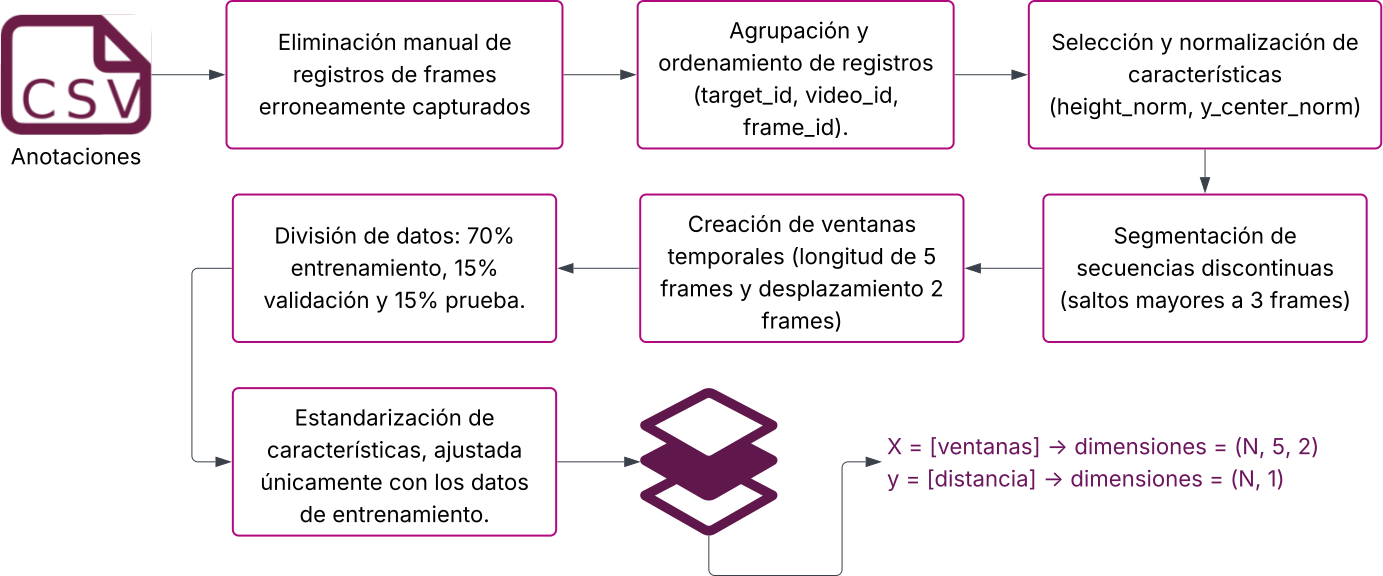
\includegraphics[width=\linewidth]{images/metodologia/preprocess_data.pdf}
    \caption{Etapas de tratamiento de las anotaciones}
    \label{fig:diag_preprocess}
\end{figure}

\subsubsection{Depuración de datos}

Durante la inspección de calidad de las anotaciones se observó que existieron errores de identificación y seguimiento provistos por el algoritmo DeepSORT (ver Fig.\ref{fig:diag_etiquetado}). Esto debido a que, ante oclusiones o cambios bruscos en la apariencia o posición, el algoritmo prioriza la asociación que minimiza su costo interno (apariencia + predicción del filtro Kalman), lo que puede conducir a confundir detecciones cercanas. Estas reasignaciones dieron lugar a distancias anotadas que no correspondían al sujeto objetivo.\\
Para detectar estos fallos se generaron versiones del video con las anotaciones (bbox, identificador de track y distancia anotada) superpuestas por cada target; esta revisión visual inicial permitió localizar y contextualizar los instantes en que las anotaciones resultaban incongruentes con la distancia conocida del sujeto.\\ 
A partir de esta referencia visual, la depuración consistió en verificar, 

\subsubsection{Análisis de datos}

A continuación, debido a la naturaleza secuencial de las redes recurrentes, se realizó la agrupación de los datos por medio del identificador de la persona y del video, esto con el fin de evitar que el modelo fuera entrenado con una secuencia que saltara de una persona a otra. 

El paso siguiente fue la selección de las características, con base en los datos proporcionados, las características relevantes tomadas fueron: la coordenada vertical del punto central del cuadro envolvente y la altura de éste recuadro. La normalización consistió en dividir dichos valores entre 1080 (altura en pixeles del frame); de tal forma que se pasa de tener las características en pixeles a tenerlas en valores de 0 a 1. 

Debido a la previa eliminación de frames con datos erróneos, la secuencia de imágenes pudo haber perdido su consistencia temporal, para corregir esto se realizaron segmentaciones; lo anterior consiste en verificar si la secuencia perdió más de 3 frames durante la limpieza de datos, y de ser así se divide la secuencia en dos diferentes, con el punto de corte justo en la posición de la pérdida de frames. Al finalizar este proceso se obtienen múltiples cadenas de frames con una correcta consistencia temporal.

Las redes neuronales recurrentes reciben secuencias de información para predecir el valor final; por lo tanto, se utiliza un tamaño de ventana que define cuántos valores va a recibir la red por cada muestra. El tamaño de ventana propuesto es de cinco valores, de cada secuencia original se tomarán esos cinco valores y se seleccionarán con un desplazamiento de dos frames hacia adelante. Además, lo anterior permite aumentar el numero de muestras, de acuerdo a la Eq.\ref{eq:n_ventanas} y mantener la dinámica temporal de la secuencia.

\begin{equation}
    N_{\text{ventanas}} = \left\lfloor \frac{L - \text{longitud\_ventana}}{\text{desplazamiento}} \right\rfloor + 1
    \label{eq:n_ventanas}
\end{equation}

Finalmente se realizó la división del conjunto de entrenamiento en un 70 porciento y 15 porciento tanto para validación como para prueba. Dentro del conjunto de entrenamiento se forzó a que los datos del individuo con la menor altura (1.51) estuvieran presentes. Con los datos de entrenamiento se ajustó la estandarización de características y se aplicaron a los demás subconjuntos.
Cada muestra tiene una dimensión de (5,2), correspondiente a 5 frames y dos características cada uno, por otro lado, el objetivo (\textit{target}) es la distancia correspondiente al último \textit{frame} en milímetros.

\subsection{Modelo de red neuronal recurrente híbrida}
\begin{figure}
    \centering
    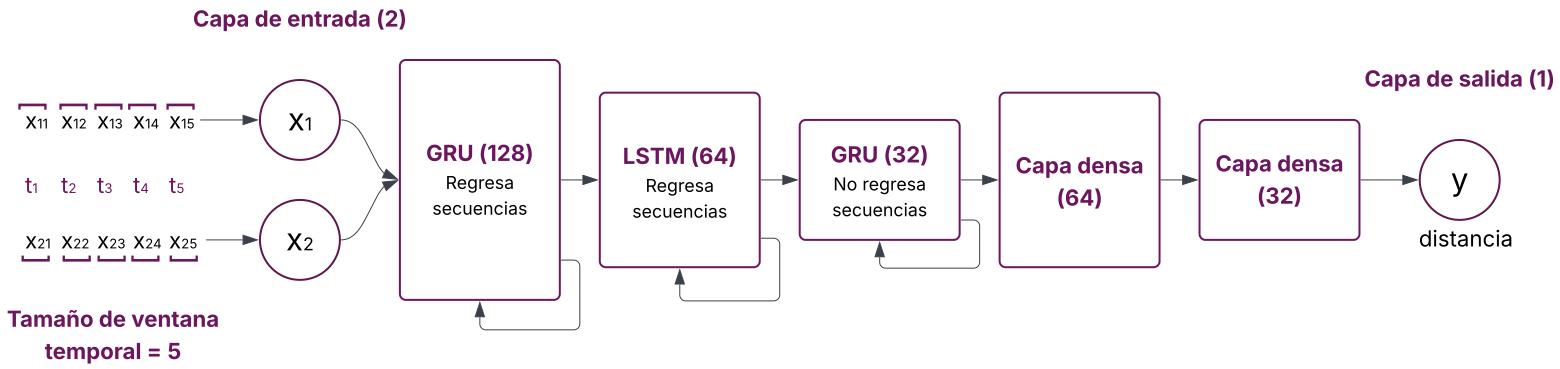
\includegraphics[width=\linewidth]{images/metodologia/nn_diagram.pdf}
    \caption{Arquitectura de la RNN híbrida}
    \label{fig:diag_nn}
\end{figure}

Debido a la naturaleza secuencial de los datos, se propone una arquitectura de red con capas de LSTM y GRU (ver Fig.\ref{fig:diag_nn}). Se tiene una entrada temporal de dos variables seguida de dos capas recurrentes y dos densas con una salida de una sola unidad. Las capas recurrentes utilizan la función de activación \texttt{tanh} para las activaciones principales y \texttt{sigmoid} para las demás, mientras que en las capas intermedias densas se utiliza \texttt{ReLU} y en la capa de salida la función \texttt{lineal}.

La función de pérdida utilizada es el error cuadrático medio (\texttt{MSE}) con el optimizador \texttt{Adam}; adicionalmente se monitorea también el error absoluto medio \texttt{MAE}. Con respecto a la regularización, se aplica \texttt{L2} de $5 \times 10^{-5}$  en las primeras dos capas recurrentes y de $1 \times 10^{-4}$ en las capas densas; se aplica \texttt{dropout} de $0.15$ para las primeras dos capas recurrentes y para las capas densas $0.25$ y $0.15$ respectivamente; también se implementaron mecanismos de regularización adaptativa mediante \texttt{EarlyStopping} y \texttt{ReduceLROnPlateau} de Keras. Las métricas de evaluación registradas son \texttt{MAE}, \texttt{MSE}, \texttt{RMSE}, \texttt{$R^{2}$}, \texttt{MAPE} y \texttt{$\sigma(AE)$}.

\newpage
\section{Resultados}
\label{cap-result}

En esta sección se presentan los resultados obtenidos al evaluar las dos variantes de la red recurrente (GRU y LSTM) entrenadas bajo la configuración descrita previamente. Primero se muestran las curvas de entrenamiento para comprobar la convergencia (ver Fig \ref{fig:training_curves}); a continuación, se reportan las métricas agregadas en \emph{test} y se realiza un análisis de error detallado: distribución global (ver Tabla \ref{tab:metrics_comparison}) y por rangos de distancia (ver Fig \ref{fig:results_gru_lstm}). Finalmente se muestran ejemplos cualitativos y una discusión sobre el comportamiento observado.
\subsection{Dinámica de entrenamiento}
La figura \ref{fig:training_curves} muestra la evolución de la pérdida (MSE) durante el entrenamiento de ambas variantes (GRU a la izquierda y LSTM a la derecha). Se observa una caída pronunciada de la pérdida en las primeras épocas seguida de una meseta intermedia y una nueva reducción posterior. 
\begin{figure}[H]
  \centering
  \includegraphics[width=0.48\linewidth]{images/resultados/GRULoss.png}
  \includegraphics[width=0.48\linewidth]{images/resultados/LSTMLoss.png}
  \caption{Evolución de la pérdida (MSE) durante el entrenamiento para GRU (izquierda) y LSTM (derecha).}
  \label{fig:training_curves}
\end{figure}

Proponemos como hipótesis que este comportamiento en dos fases está relacionado con la naturaleza estocástica del entrenamiento y con la forma en que se construyen los mini-batches. En una primera etapa, el modelo aprende patrones generales y la pérdida desciende rápidamente; después aparece una meseta cuando las actualizaciones dejan de producir mejoras claras. Con el paso de las épocas, la variación entre batches —así como la posible agrupación de ejemplos por \emph{target\_id}— introduce suficiente diversidad como para que el optimizador salga de ese estancamiento y logre una segunda etapa de refinamiento. \\
Otro aspecto relevante observado durante el entrenamiento fue la diferencia en convergencia y tiempo entre las dos variantes. El modelo GRU alcanzó su mejor validación mucho antes (época 51) que la LSTM (época 115), lo que indica una convergencia más rápida en las condiciones experimentales usadas. Por otra parte, la LSTM alcanzó un mejor `val\_mae` final (0.5016 m frente a 0.5288 m para la GRU), a costa de más épocas y mayor tiempo por época. Estas diferencias pueden presentarse debido a las características internas de cada bloque recurrente (capacidad de modelado y coste computacional) como a la configuración experimental (número de unidades por bloque, batching por \emph{target\_id}, etc.).

\subsection{Evaluación en conjunto de prueba}
\subsubsection{Métricas globales}
Las métricas globales se calcularon sobre el conjunto de prueba para comparar de forma directa el desempeño de las dos variantes entrenadas (LSTM y GRU). Se reportan MAE (con su desviación estándar del error absoluto), RMSE, R$^2$, MAPE y el número de secuencias evaluadas. La tabla \ref{tab:metrics_comparison} resume los resultados obtenidos por ambos modelos.
\begin{table}[H]
\centering
\begin{tabular}{l cc}
\hline
\textbf{Métrica} & \textbf{LSTM} & \textbf{GRU} \\
\hline
MAE (m) & $0.7106 \pm 0.6116$ & $0.7358 \pm 0.5726$ \\
RMSE (m) & $0.9376$ & $0.9324$ \\
R$^2$ & $0.9792$ & $0.9794$ \\
MAPE (\%) & $4.11$ & $4.30$ \\
\hline
\end{tabular}
\caption{Comparativa de métricas globales en el conjunto de prueba para las variantes LSTM y GRU.}
\label{tab:metrics_comparison}
\end{table}

La LSTM muestra un MAE y un MAPE ligeramente mejores que la GRU, mientras que la GRU presenta un RMSE marginalmente menor y un R$^2$ prácticamente idéntico. Las diferencias son pequeñas en magnitud.

\subsubsection{Visualización de resultados}
A continuación, en la Figura~\ref{fig:results_gru_lstm} se presentan las visualizaciones principales que permiten analizar el comportamiento de ambas variantes en el conjunto de prueba. Estas figuras complementan las métricas numéricas previamente reportadas y ofrecen una vista directa sobre la relación entre las predicciones y los valores reales, así como sobre la distribución y magnitud de los errores obtenidos para cada arquitectura.
\begin{figure}[H]
  \centering

  % --- Fila 1: GRU ---
  \begin{subfigure}{0.32\textwidth}
    \centering
    \includegraphics[width=\linewidth]{images/resultados/aGRU.png}
    \caption{}
    \label{subfig:gru_pred_vs_real}
  \end{subfigure}\hfill
  \begin{subfigure}{0.32\textwidth}
    \centering
    \includegraphics[width=\linewidth]{images/resultados/bGRU.png}
    \caption{}
    \label{subfig:gru_err_hist}
  \end{subfigure}\hfill
  \begin{subfigure}{0.32\textwidth}
    \centering
    \includegraphics[width=\linewidth]{images/resultados/cGRU.png}
    \caption{}
    \label{subfig:gru_abs_err_hist}
  \end{subfigure}

  \vspace{6pt} % espacio entre filas

  % --- Fila 2: LSTM ---
  \begin{subfigure}{0.32\textwidth}
    \centering
    \includegraphics[width=\linewidth]{images/resultados/dLSTM.png}
    \caption{}
    \label{subfig:lstm_pred_vs_real}
  \end{subfigure}\hfill
  \begin{subfigure}{0.32\textwidth}
    \centering
    \includegraphics[width=\linewidth]{images/resultados/eLSTM.png}
    \caption{}
    \label{subfig:lstm_err_hist}
  \end{subfigure}\hfill
  \begin{subfigure}{0.32\textwidth}
    \centering
    \includegraphics[width=\linewidth]{images/resultados/fLSTM.png}
    \caption{}
    \label{subfig:lstm_abs_err_hist}
  \end{subfigure}

  \caption{Comparativa visual del desempeño en test: fila superior = GRU; fila inferior = LSTM. (a)/(d) Predicción vs.\ Real con línea identidad; (b)/(e) histograma de errores (\( \text{Pred} - \text{Real} \)); (c)/(f) histograma de errores absolutos.}
  \label{fig:results_gru_lstm}
\end{figure}

A partir de estas representaciones se puede contrastar directamente el comportamiento de ambas arquitecturas. \\
En términos del análisis de la alineación entre las predicciones y los valores reales, las subfiguras~\ref{subfig:gru_pred_vs_real} y~\ref{subfig:lstm_pred_vs_real} permiten observar que tanto el modelo GRU como el de LSTM siguen una tendencia cercana a la línea identidad, lo que indica que, en general, el modelo logra replicar adecuadamente la progresión de distancias del conjunto de prueba. La GRU muestra una dispersión un poco mayor, especialmente en distancias altas, mientras que la LSTM mantiene un agrupamiento ligeramente más consistente alrededor de la referencia. En esta última también se aprecia una leve subestimación en el intervalo aproximado de 2–3 m, aunque se trata de un efecto reducido.\\
Las distribuciones de error presentadas en las subfiguras correspondientes (ver Fig.~\ref{subfig:gru_err_hist}, \ref{subfig:lstm_err_hist}) muestran una forma aproximadamente gaussiana centrada en valores cercanos a cero, lo que sugiere ausencia de sesgos marcados y estabilidad general en las predicciones. En la variante GRU, la media del error es \(\mu = -0.348\,\text{m}\) y su dispersión alcanza \(\sigma = 0.865\,\text{m}\), reflejando una leve subestimación acompañada de una variabilidad moderada. Por otra parte, la LSTM presenta una media aún más próxima a cero, \(\mu = -0.218\,\text{m}\), junto con una desviación estándar ligeramente mayor, \(\sigma = 0.912\,\text{m}\).\\
En las distribuciones de errores absolutos mostradas en las subfiguras \ref{subfig:gru_abs_err_hist} y \ref{subfig:lstm_abs_err_hist} permiten evaluar la magnitud típica de las desviaciones en las predicciones. En ambos modelos se observa una concentración alta de valores por debajo de 1\,m, lo que indica que la mayoría de las estimaciones se mantienen dentro de un rango de error reducido. En la GRU, la mayor concentración de valores se agrupa ligeramente más cerca del origen, reflejando su MAE de menor magnitud. En la LSTM, aunque también predomina la zona de errores pequeños, la cola de la distribución se extiende un poco más, consistente con la presencia ocasional de errores absolutos mayores.

\subsection{Inferencia del modelo sobre videos}
\begin{figure}[H]
    \centering
    % Subfigura superior izquierda
    \begin{subfigure}{0.45\textwidth}
        \centering
        \includegraphics[width=\linewidth]{images/resultados/modelo_vid_1.png} \\
        \label{subfig:vid-1}
    \end{subfigure}
    \hfill
    % Subfigura superior derecha
    \begin{subfigure}{0.45\textwidth}
        \centering
        \includegraphics[width=\linewidth]{images/resultados/modelo_vid_2.png} \\
        \label{subfig:vid-2}
    \end{subfigure}

    \vspace{0.5cm} % Espacio entre las filas de imágenes

    % Subfigura inferior izquierda
    \begin{subfigure}{0.45\textwidth}
        \centering
        \includegraphics[width=\linewidth]{images/resultados/modelo_vid_3.png} \\
        \label{subfig:vid-3}
    \end{subfigure}
    \hfill
    % Subfigura inferior derecha
    \begin{subfigure}{0.45\textwidth}
        \centering
        \includegraphics[width=\linewidth]{images/resultados/modelo_vid_4.png} \\
        \label{subfig:vid-4}
    \end{subfigure}

    \caption{Frames de resultado tras aplicar el modelo de red neuronal sobre videos}
    \label{fig:result_videos}
\end{figure}


\newpage
\section{Conclusiones}
Durante esta etapa del proyecto se ha avanzado en la exploración de modelos auto-supervisados de estimación de profundidad monocular. Estos modelos han permitido comprender mejor el funcionamiento y limitaciones de este tipo de enfoques, especialmente en lo relativo a la ambigüedad de escala y su comportamiento en entornos no controlados. Si bien han mostrado resultados prometedores en contextos específicos, también han evidenciado que la precisión de las estimaciones puede degradarse significativamente ante cambios de iluminación, geometría compleja o variaciones en la dinámica de la escena.

De este modo, se ha fortalecido la estructura metodológica del proyecto, incluyendo la planificación para la generación de un dataset propio y la evaluación inicial de modelos de última generación como DepthAnything, cuya arquitectura y rendimiento lo posicionan como un candidato prometedor para el caso de estudio. Este modelo ha sido probado de manera preliminar, lo que ha permitido obtener una visión más clara sobre su potencial y sobre los desafíos que aún deben resolverse.

Aunque los modelos analizados hasta ahora ofrecen una base interesante para abordar el problema, aún se requiere un trabajo más profundo tanto en la experimentación como en la integración de múltiples enfoques para abordar de forma más robusta las condiciones reales del entorno. Estos avances metodológicos y conceptuales constituyen una base sólida para continuar con las siguientes fases del proyecto.

% Referencias
\newpage
\bibliographystyle{plainnat}
\bibliography{referencias}
\addcontentsline{toc}{section}{Referencias}

\end{document}